\chapter{Evaluation}
\label{chapter:evaluation}

\section{Calibration quality}
For computing the error of each camera calibration, another tool from the same ROS Camera Calibration package is used.
It outputs a reprojection $\mathsf{RMS}$ error, which stands for Root-mean-square error and can be defined as
\begin{equation}
    \mathsf{RMS}(x) = \sqrt{\frac{\sum_{i=1}^{N}{(x_i - \hat{x}_i)^2}}{N}}
\end{equation}
where $x$ is a measured data sample from the experiment, $\hat{x}$ is a ground-truth data and $N$ is a sample size.
The reprojection error varies depending on the pose of the chessboard, but in general is quite stable, see \autoref{tab:camcalib_eval}.

\begin{table}[ht]
    \begin{center}
      \begin{tabular}{ ll l l }
      \hline
      && Left camera & Right camera \\ \hline
      mean of RMS reprojection error & [px] & 0.06323214286 & 0.05357391304 \\
      variance of RMS reprojection error & [px] & 0.00001159968 & 0.00002222914 \\
      \end{tabular}
    \end{center}
    \caption{ROS Camera Calibration results.}
    \label{tab:camcalib_eval}
\end{table}

\section{Triangulation quality}
There were two experiments to measure the triangulation quality.
The same image with visible key points in a featureless environment was used.

\subsection{Experiment setup}
\label{sec:eval_setup}

\begin{figure}[ht]
  \begin{subfigure}[ht]{0.29\textwidth}
    \centering
    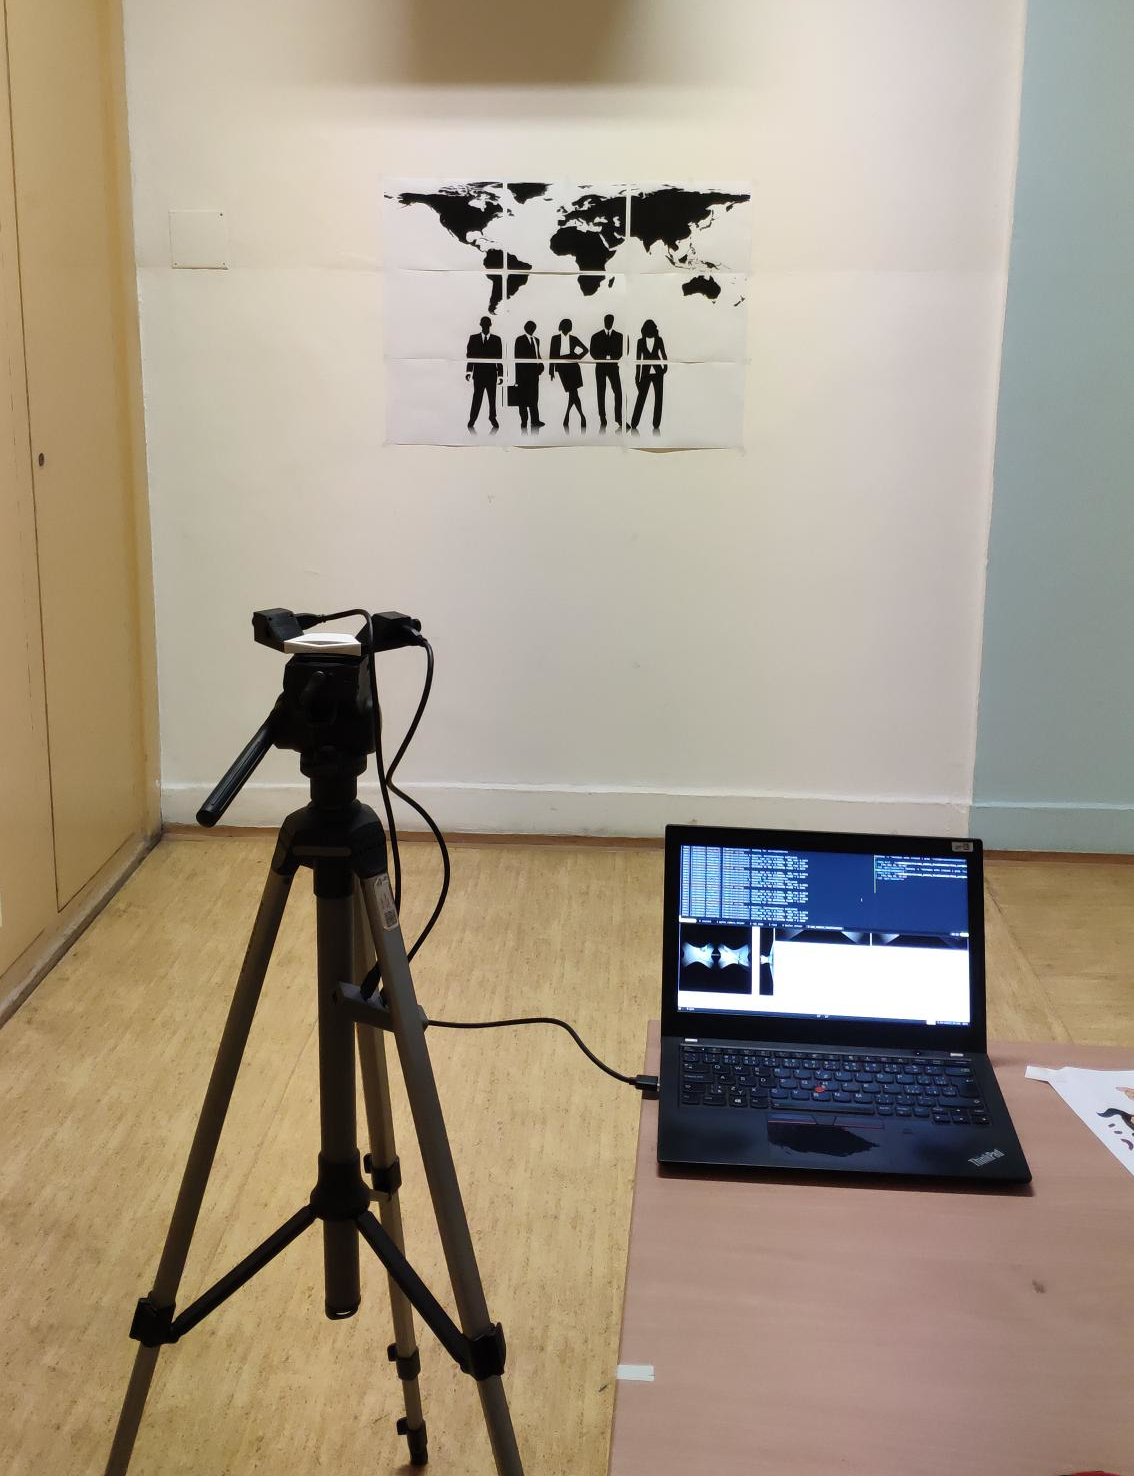
\includegraphics[width=\textwidth]{graphics/experiment_setup.png}
    \caption[The setup for experiments]{The setup for experiments. 
    The designed prototype is located on a tripod, on a distance $d$ from the plane with features, with y-z plane parallel to the $\Omega$. 
    A set of 9 A4 papers with features was used to make $\Omega$ distinguishable.}
    \label{fig:exp_process}
  \end{subfigure}
  \hfill
  \begin{subfigure}[ht]{0.7\textwidth}
    \centering
    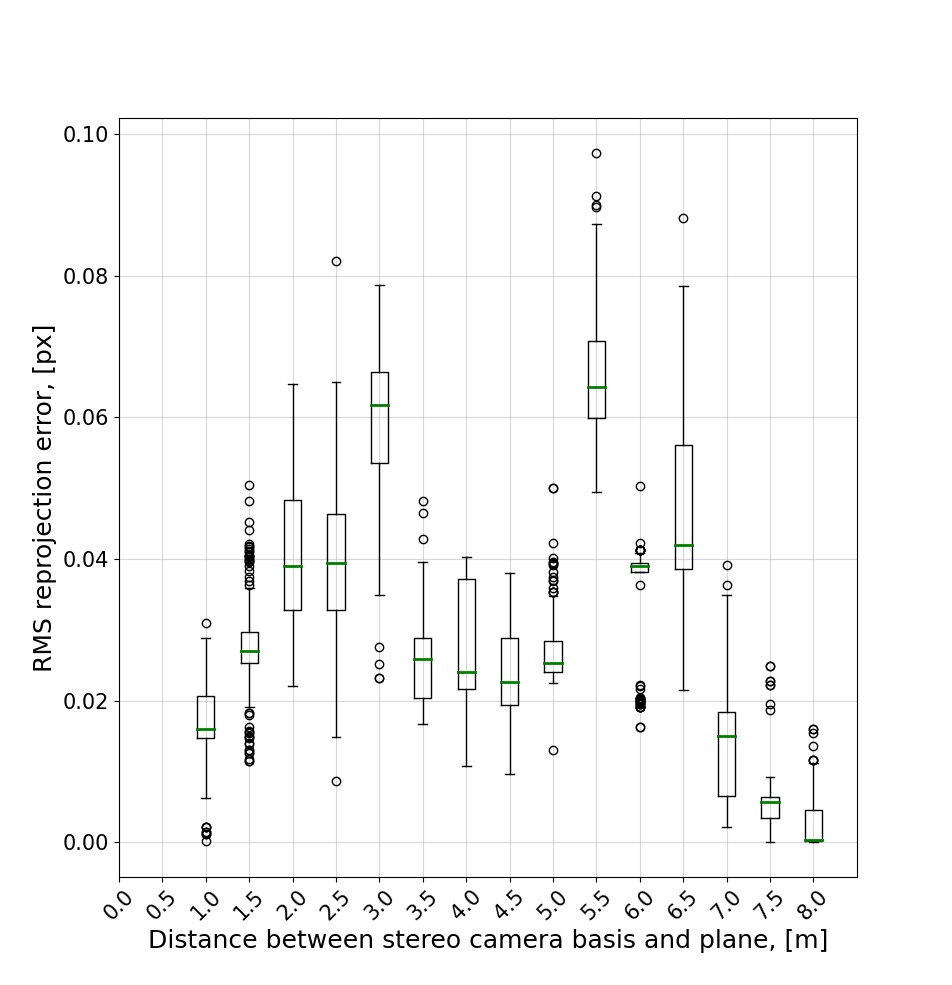
\includegraphics[width=\textwidth]{graphics/experiment_1_repro_error.png}
    \caption[Stereopair calibration RMS reprojection error.]{Stereopair calibration RMS reprojection error. Red line represents the trend of the sample.}
    \label{fig:exp_1_repro}
  \end{subfigure}
  \caption{The experiment setup and reprojection error measurements.}
  \label{fig:exp_1_exp0}
\end{figure}

\begin{figure}[ht]
  \begin{subfigure}[ht]{0.49\textwidth}
    \centering
    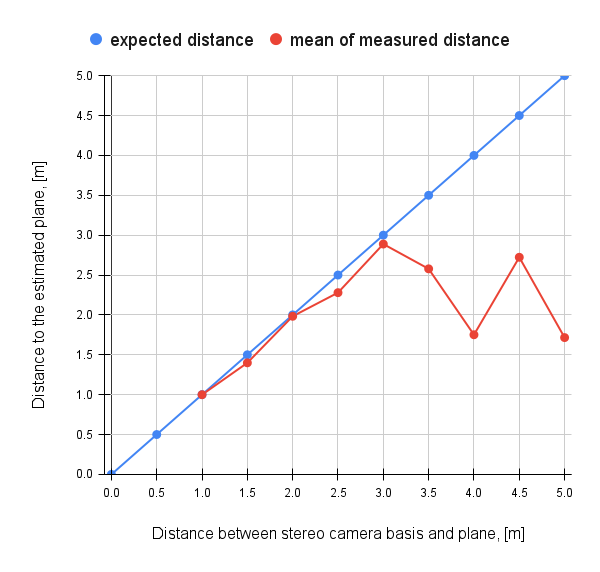
\includegraphics[width=\textwidth]{graphics/experiment_1_chart_planedist.png}
    \caption[Distance to the estimated plane]{Distance $d$ from the stereo camera to $\Omega$.
    Blue line represents the expected distance, and red line represents $d'$, compute as mean of $n$ estimated distances.}
    \label{fig:exp_1_chart_dists}
  \end{subfigure}
  \hfill
  \begin{subfigure}[ht]{0.49\textwidth}
    \centering
    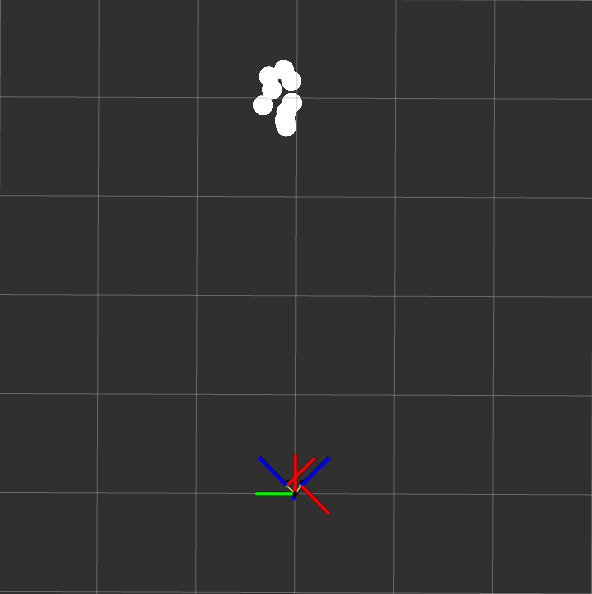
\includegraphics[width=\textwidth]{graphics/experiment_1_4m.png}
    \caption[The experiment top view]{The experiment top view. 
    The grid's cell size is $1$m$\times$$1$m.
    The cololred axis represents basis of individual cameras and the stereo camera basis.
    Red color stands for $X$ coordinate, green for $Y$ and blue for $Z$.
    The basis aligned with the grid represents the stereo camera basis, $X$ axis towords the point cloud.
    The point cloud (white dots) represents reconstructed feature points seen by both cameras.}
    \label{fig:exp_1_topview}
  \end{subfigure}
  \caption{The first experiment results: distance to the estimated plane.}
  \label{fig:exp_1_exp}
\end{figure}

\begin{figure}[ht]
  \begin{subfigure}[ht]{.49\textwidth}
    \centering
    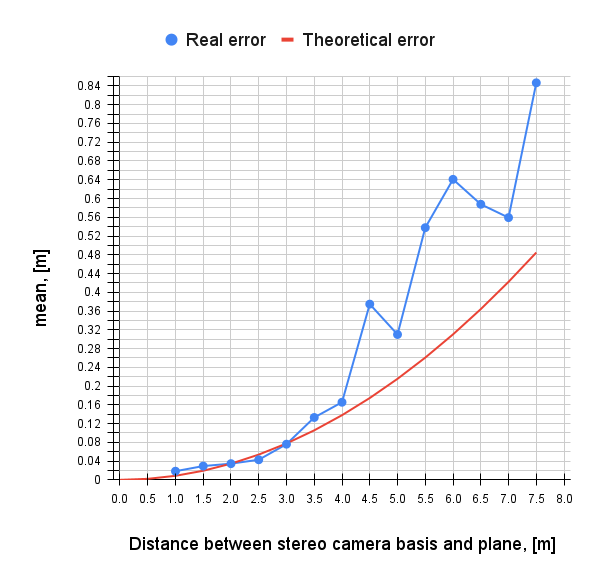
\includegraphics[width=\textwidth]{graphics/exp2_mean.png}
    \caption{Second experiment. Mean of $e'_i$.}
    \label{fig:exp_2_mean}
  \end{subfigure}
  \hfill
  \begin{subfigure}[ht]{0.49\textwidth}
    \centering
    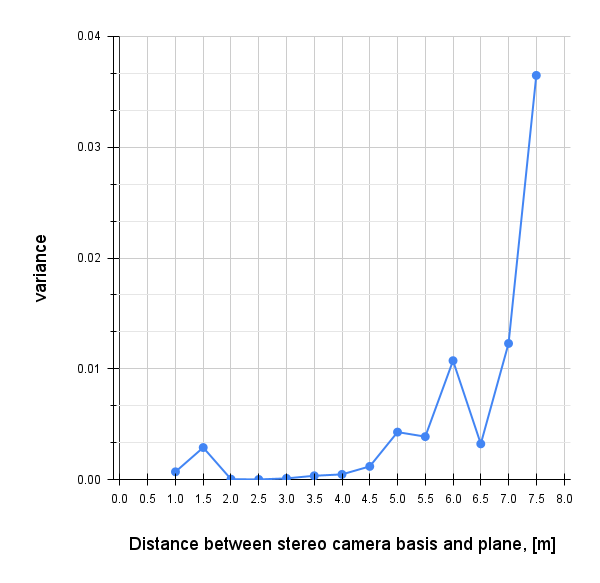
\includegraphics[width=\textwidth]{graphics/exp2_var.png}
    \caption{Second experiment. Variance of $e'_i$.}
    \label{fig:exp_2_var}
  \end{subfigure}
  \begin{subfigure}[b]{\textwidth}
      \centering
      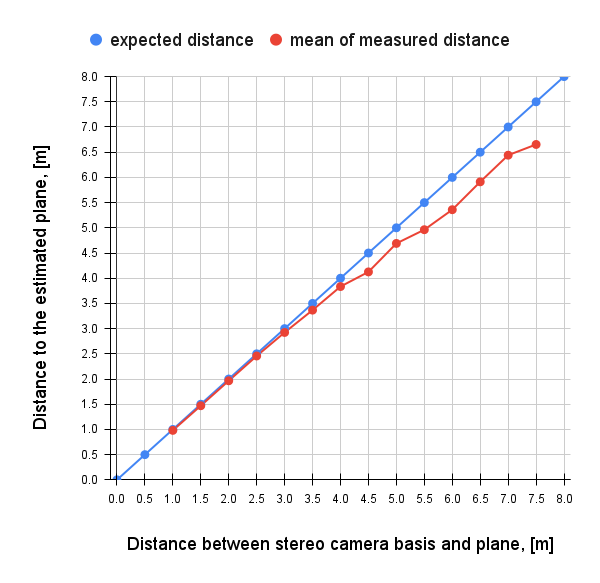
\includegraphics[width=0.5\textwidth]{graphics/experiment_2_chart_planesist.png}
      \caption{Second experiment. Distance from the stereo camera to the estimated plane.
      Blue line represents the expected distance $d$, and red line represents $d'$, computed as mean of $n$ estimated distances, where each $d'_{i}$ is defined as average distance from points in time $i$ to the given plane $\Omega$.}
      \label{fig:exp_2_res}
  \end{subfigure}
  \caption{The second experiment results: distance to the predefined plane.}
  \label{fig:exp_2_}
\end{figure}

One possible approach to evaluate the quality of triangulation is to have the environment with all key points on one plain.
Reprojection error is not entirely representative here because, with the distance increasing, the key points are clustered, and the reprojection error decreases (see \autoref{fig:exp_1_repro}).
To measure the quality of distance estimation, the following approach was chosen.
The image with multiple features was attached to the white wall in a corridor with a featureless environment to reduce the noise.
The camera prototype on a tripod was located at a fixed distance from the wall to have its setup y-z plane parallel to the wall as in \autoref{fig:exp_process}.

Let us define the wall plane as $\Omega$, distance from stereo camera basis to the wall as $d$, estimated plane as $\Omega'$ and estimated distance to the plane as $d'$.
The number of timestamps for each experiment is $n=120$, and $i$ is a timestamp index, $i \in \{1 \dots 120\}$.

\subsection{Distance to the estimated plane}
\label{sec:exp1}
After 3D points are computed, the plane passing through them is estimated with RANSAC using PCL implementation. 
The absolute difference between the distance from the camera to the computed plane and the distance from the camera to the wall plane is taken as the error.

The distance $d$ for this experiment was from $1$m to $5$m with a step of $0.5$m.
The result of this experiment is shown in \autoref{fig:exp_1_chart_dists}.
According to the figure, the distance deviates significantly after $3.5$m.
In \autoref{fig:exp_1_topview} the topview of the experiment is shown for $d=4$m.
It can be seen that the plane can not be estimated correctly at this distance because of a small error for each triangulated point.

\subsection{Distance to the predefined plane}
\label{sec:exp2}
With increasing the distance $d$, feature points became less distinguishable due to resolution bounds.
In \autoref{fig:exp_process} triangulated points do not define a plane, but still, they are close to the actual plane.
That is why the second experiment was constructed.

The experiment was done using the same setup as in \autoref{sec:eval_setup}. 
The difference is that $\Omega'$ is compute not using the RANSAC to fit the plane between points, but as the plane parallel to $\Omega$ on a distance $e'_i$, that can be defined as
\begin{equation}    
    e'_i = \frac{1}{k} \sum_{j=0}^{k}{|p'_j|},
\end{equation}
where $k$ is the number of keypoints detected at a timestamp $t_i$, and $p'_j$ is the distance from point $\vec{p}'_j$ to $\Omega$.
Then $d'_i$ is defined as 
\begin{equation}
    d'_i = d_i - e'_i.
\end{equation}

The distance $d$ was from $1$m to $7.5$m as the maximum distance at which key points can be detected (empirically found) with the step of $0.5$m.
The mean and variance of $e'_i$ is shown in \autoref{fig:exp_2_mean} and \autoref{fig:exp_2_var}, and comparison of $d_i$ and $d'_i$ is in \autoref{fig:exp_2_res}. 

\section{Rate testing}
\begin{table}[ht]
    \begin{center}
      \begin{tabular}{lll}
      \hline
        Parameter & & Value \\
        Minimal delay over 5min & [s]  & 10.607 \\
        Maximal delay over 5min & [s]  & 0.042 \\
        Average rate over 5min  & [Hz] & 0.196 \\ 
      \end{tabular}
    \end{center}
    \caption{Proposed system working frequency.}
    \label{tab:eval_freq}
\end{table}

To ensure that obstacles can be detected, not only triangulation quality is important, but also the speed with which the MAV can receive the data from the obstacle avoidance module and the frequency of a system.
The working frequency, max and min delays are shown in \autoref{tab:eval_freq}.
 
\section{Experiments summary}
The quality of distance estimation to obstacles was shown in both experiments.
The first experiment, described in \autoref{sec:exp1}, shows that the precision of a proposed method is relatively high for distances up to 3m, and the second experiment, described in \autoref{sec:exp2} only proved it. 
The estimated distance error on $3$m is less than $3\%$.
The maximum available distance to detect points is $7.5$m with an error up to $1$m.
On further distances, key points can not be detected anymore due to the camera resolution and focal length (cameras were calibrated on distances up to $2$m).
The proposed solution works with the average frequency of $TODO$Hz.
